\documentclass{article}

% if you need to pass options to natbib, use, e.g.:
%     \PassOptionsToPackage{numbers, compress}{natbib}
% before loading neurips_2021

% ready for submission
\usepackage[final]{neurips_2021}

% to compile a preprint version, e.g., for submission to arXiv, add add the
% [preprint] option:
%     \usepackage[preprint]{neurips_2021}

% to compile a camera-ready version, add the [final] option, e.g.:
%     \usepackage[final]{neurips_2021}

% to avoid loading the natbib package, add option nonatbib:
%    \usepackage[nonatbib]{neurips_2021}

\usepackage[utf8]{inputenc} % allow utf-8 input
\usepackage[T1]{fontenc}    % use 8-bit T1 fonts
\usepackage{hyperref}       % hyperlinks
\usepackage{url}            % simple URL typesetting
\usepackage{booktabs}       % professional-quality tables
\usepackage{amsfonts}       % blackboard math symbols
\usepackage{nicefrac}       % compact symbols for 1/2, etc.
\usepackage{microtype}      % microtypography
\usepackage{xcolor}         % colors
\usepackage{graphicx}
\usepackage{float}
\usepackage{makecell}
\usepackage{multicol}

\title{Snakes 3v3: VI or DQN?}

% The \author macro works with any number of authors. There are two commands
% used to separate the names and addresses of multiple authors: \And and \AND.
%
% Using \And between authors leaves it to LaTeX to determine where to break the
% lines. Using \AND forces a line break at that point. So, if LaTeX puts 3 of 4
% authors names on the first line, and the last on the second line, try using
% \AND instead of \And before the third author name.

\author{%
  Keyao You \\
  Shanghai Jiao Tong University \\
  \texttt{youkeyao@sjtu.edu.cn} \\
  % examples of more authors
   \And
   Yazhou Tang \\
   Shanghai Jiao Tong University \\
   \texttt{tangyazhou518@sjtu.edu.cn} \\
  % \AND
  % Coauthor \\
  % Affiliation \\
  % Address \\
  % \texttt{email} \\
  % \And
  % Coauthor \\
  % Affiliation \\
  % Address \\
  % \texttt{email} \\
  % \And
  % Coauthor \\
  % Affiliation \\
  % Address \\
  % \texttt{email} \\
}

\begin{document}

\maketitle

\begin{abstract}
  In this project, we need to use our own agent to beat the opponent in the Snake 3v3 game on the Jidi AI platform\footnote{http://www.jidiai.cn/compete\_detail?compete=13}. We have tried several algorithms to design our agent, like Minimax, Value Iteration, and Dueling DQN, while introducing specific strategies from the Snake game. Finally, we analyse the advantages and disadvantages of each algorithm, and choose the best-performed one.
  
\end{abstract}

\section{Introduction}

Snake 3v3 is a multiplayer game where players make decisions to control their snakes at the same time each turn (the number of snakes controlled by each player is 3).

\subsection{Problem description}

\subsubsection{Game rules}

According to information on the website, this game has several rules below.

\begin{enumerate}
    \item There are 2 players in the game, each of them will control 3 snakes.
    \item When snake's heads are in the body of its own or other snakes', this snake will be judged to be dead. It will then randomly reborn at any location on the map.
    \item When snake eats a bean, its length will increase by 1. When a bean is eaten, it will randomly be generated anywhere on the map, thus ensuring that the total number of beans on the map is 5.
    \item After 200 steps, the player with the larger sum of snakes' length wins.
\end{enumerate}

\subsubsection{Agent input and output}

We need to write a Python program called \texttt{submission.py}. Here is the input provided by the game program and the output we need to prepare.

\begin{enumerate}
    \item The first input \texttt{observation} is a dictionary with key from \texttt{1} to \texttt{7} and \texttt{board\_width}, \texttt{board\_height}, \texttt{last\_direction}, \texttt{controlled\_snake\_index}. Here, 
    
    \begin{enumerate}
        \item \texttt{1} represents beans, while \texttt{2} to \texttt{7} represent snakes.
        \item The value of the dictionary is a list with \texttt{[h,w]} coordinates as elements, representing positions of beans or snakes. \texttt{h} represents the vertical distance from the origin in the upper left corner, \texttt{w} represents the horizontal width from the origin.
        \item Among the values corresponding to \texttt{2} to \texttt{7}, the list elements from left to right represent the position of the head to the tail of the corresponding snake.
        \item The value of \texttt{board\_width} is the width of the board; The value of \texttt{board\_height} is the height of the board; The value of \texttt{last\_direction} are directions of each snake in the last step; The value of \texttt{controlled\_snake\_index} is the controlled snake index.
    \end{enumerate}
    \item The second input \texttt{action\_space} is a list of available actions.
    \item The output is the actions that our snakes will perform in this turn.
\end{enumerate}

\subsection{Problem analysis}

Our main goal is to avoid crash and let the snake eat as many beans as possible. So it is very intuitive to use adversarial search to solve this problem, or take it as a MDP problem and use value iteration to solve it. Besides, we need to mind that, we have 3 snakes instead of 1 snake, which means that it is not necessary for every controlled snake to pursue for longer length. So we have 2 kind of special cases.

\begin{itemize}
    \item \textsc{Defense}. When the snakes are too long, the possibility of crashing will increase. To avoid this kind of ``sudden death'', maybe the snakes which achieve enough length don't need to eat bean any more.
    \item \textsc{Attack}. When the snake dies in the second half of the race, it has a hard time catching up with its rivals in length again. Therefore it can move towards the opponent's head, thus increasing the probability that the opponent will collide with it.
\end{itemize}
    
When 1 or 2 snakes behave specially, others will move normally, to ensure a steady rise overall.

\section{Intuitive Algorithms}

According to the analysis above, we tried several intuitive algorithms to solve the problem.

\subsection{Minimax with $\alpha$-$\beta$ Pruning}

\subsubsection{Overview}
Since this is a multi-agent problem, we can use minimax to search the game tree and decide the action if we suppose that all snakes take the action one by one so each layer represents a snake. According to the evaluation function, we simply design it as the difference between the sum of the lengths of snakes of each party. More details are shown in the code.

\subsubsection{Result}

The result of minimax agent with random agent as opponent is shown in figure \ref{minimax-random}.

\begin{figure}[h]
  \centering
  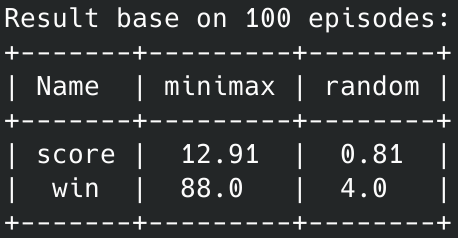
\includegraphics[width=0.5\textwidth]{figs/minimax_vs_random.png}
  \caption{minimax agent with random agent}
  \label{minimax-random}
\end{figure}

Here we set depth equal to two because it will cause a failure on Jidi platform if the depth is larger. Since minimax does not work well, we discard it and look for other methods.

\subsection{Value Iteration}

\subsubsection{Overview}
If we see each step as finding a way in a grid world, we can easily apply value iteration on it because the states are just the position in the grid world. In each step, we build a grid world in which the reward of bean and other snakes is defined by ourselves according to the observation. Then we use value iteration to count the Q value of each state and get the best policy. By the way, the reason why we do not use policy iteration is that it is a little bit slower than value iteration in this problem.

$$
V_{k+1}(s) \leftarrow \max _{a} \sum_{s^{\prime}} T\left(s, a, s^{\prime}\right)\left[R\left(s, a, s^{\prime}\right)+\gamma V_{k}\left(s^{\prime}\right)\right]
$$

\subsubsection{Special Strategies}

We use some special strategies in the Snake game solve some tricky problems, enhancing our agent.

\begin{enumerate}
    \item \textbf{Greedy problem}. The problem of this algorithm is that it is greedy to eat a bean and will easily get itself trapped. So we add a mechanism that it will follow its tail if it is long enough so that it will not die, which is a kind of defense.
    \item \textbf{Collision problem}. Due to the disability to predict other snakes' action, it is likely to collide with other snakes' head. So we also give the surroundings of other snake' head a negative reward.
    \item \textbf{Dead end problem}. This algorithm also has a problem of getting into a dead end if there is a bean in it. So we will change the bean reward to a negative value if three sides of it are snakes.
    \item \textbf{Attack action}. If the score is too low, the snake will take the attack action which means they will rush to the surrounding of opponent snakes' heads. We just give the surroundings of opponent snake' head a positive reward.
\end{enumerate}


\subsubsection{Result}
Its performance is shown in figure \ref{vi-rl}. Here we use the provided DDPG algorithm to train 50,000 episodes to get a model as our opponent, called ``RL''.

\begin{figure}[h]
  \centering
  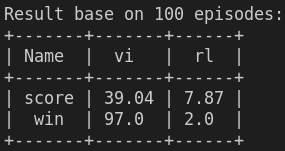
\includegraphics[width=0.5\textwidth]{figs/vi_vs_rl.png}
  \caption{VI agent with RL agent}
  \label{vi-rl}
\end{figure}

\section{Dueling DQN}

Although we used the VI algorithm to get a win rate of over 90\% in the difficulty-boosting warm-up, we believe that we can use neural networks in combination with reinforcement learning to further improve the win rate.

\subsection{Overview}
If we see the problem as a classic MDP problem, then the state space will be too large which is difficulty to store the Q value table. So we use deep Q network to learn the Q table and map environment states to actions. To make the training more stable, there are two separate Q network. The target network is frozen during training and copied from evaluation network after several steps. What's more, all training samples are put into the replay buffer and training is performed on random samples from the replay buffer so that the relevance between samples is reduced. More details are shown in our code.

But the classic DQN has a problem of overestimating the Q value, so we use dueling DQN instead. It just splits the Q value into two parts, the state value and the advantage value. The state value reflects the value of the state and the advantage value reflects the value of each action. The advantage value is restricted to have an average value of 0 so that the Q value will be more appropriate.

\subsection{Implementation}

\subsubsection{Input}
The input is designed as a $3\times 20 \times 20$ matrix. The first $20\times 20$ matrix is the position of the controlled snake. The second $20 \times 20$ matrix is the position of other snakes. The third $20 \times 20$ matrix is the position of beans. The reason why the size is $20\times 20$ instead of $10\times 20$ is that the calculation of convolution performs better on $20\times 20$ so we extend it. To show the possible moving of snakes, we also mark the surrounding of snakes' heads. To reduce the size of state space, we make the position of the controlled snake's head unchanged. The position of other snakes are calculated based on it.

\subsubsection{Network design}
We use two convolutional layers first since the input is image based. Then followed by a fully connected layer. The last layer is split to the state value function and the advantage value function. Finally combine them into the Q value. All activation functions use ReLU function. The network is shown in the figure \ref{network}.

\begin{figure}[h]
  \centering
  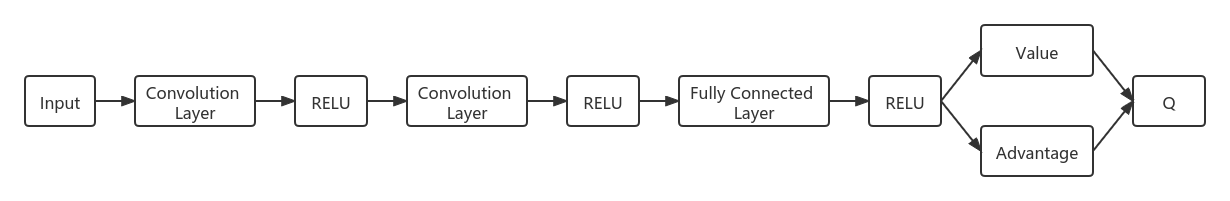
\includegraphics[width=1\textwidth]{figs/network.png}
  \caption{Network design}
  \label{network}
\end{figure}

\subsection{Training}

We have tried many times to train the model. Here we have selected two representative attempts.

In one attempt, we first use random agent to train it. After it has learned enough, we change the opponent to RL agent. Finally we train it with itself to have a better performance. The reward and win rate during training are shown in figure \ref{rw1} and figure \ref{wr1}.

\begin{figure}[H]
    \centering
    \begin{minipage}[t]{0.48\textwidth}
        \centering
        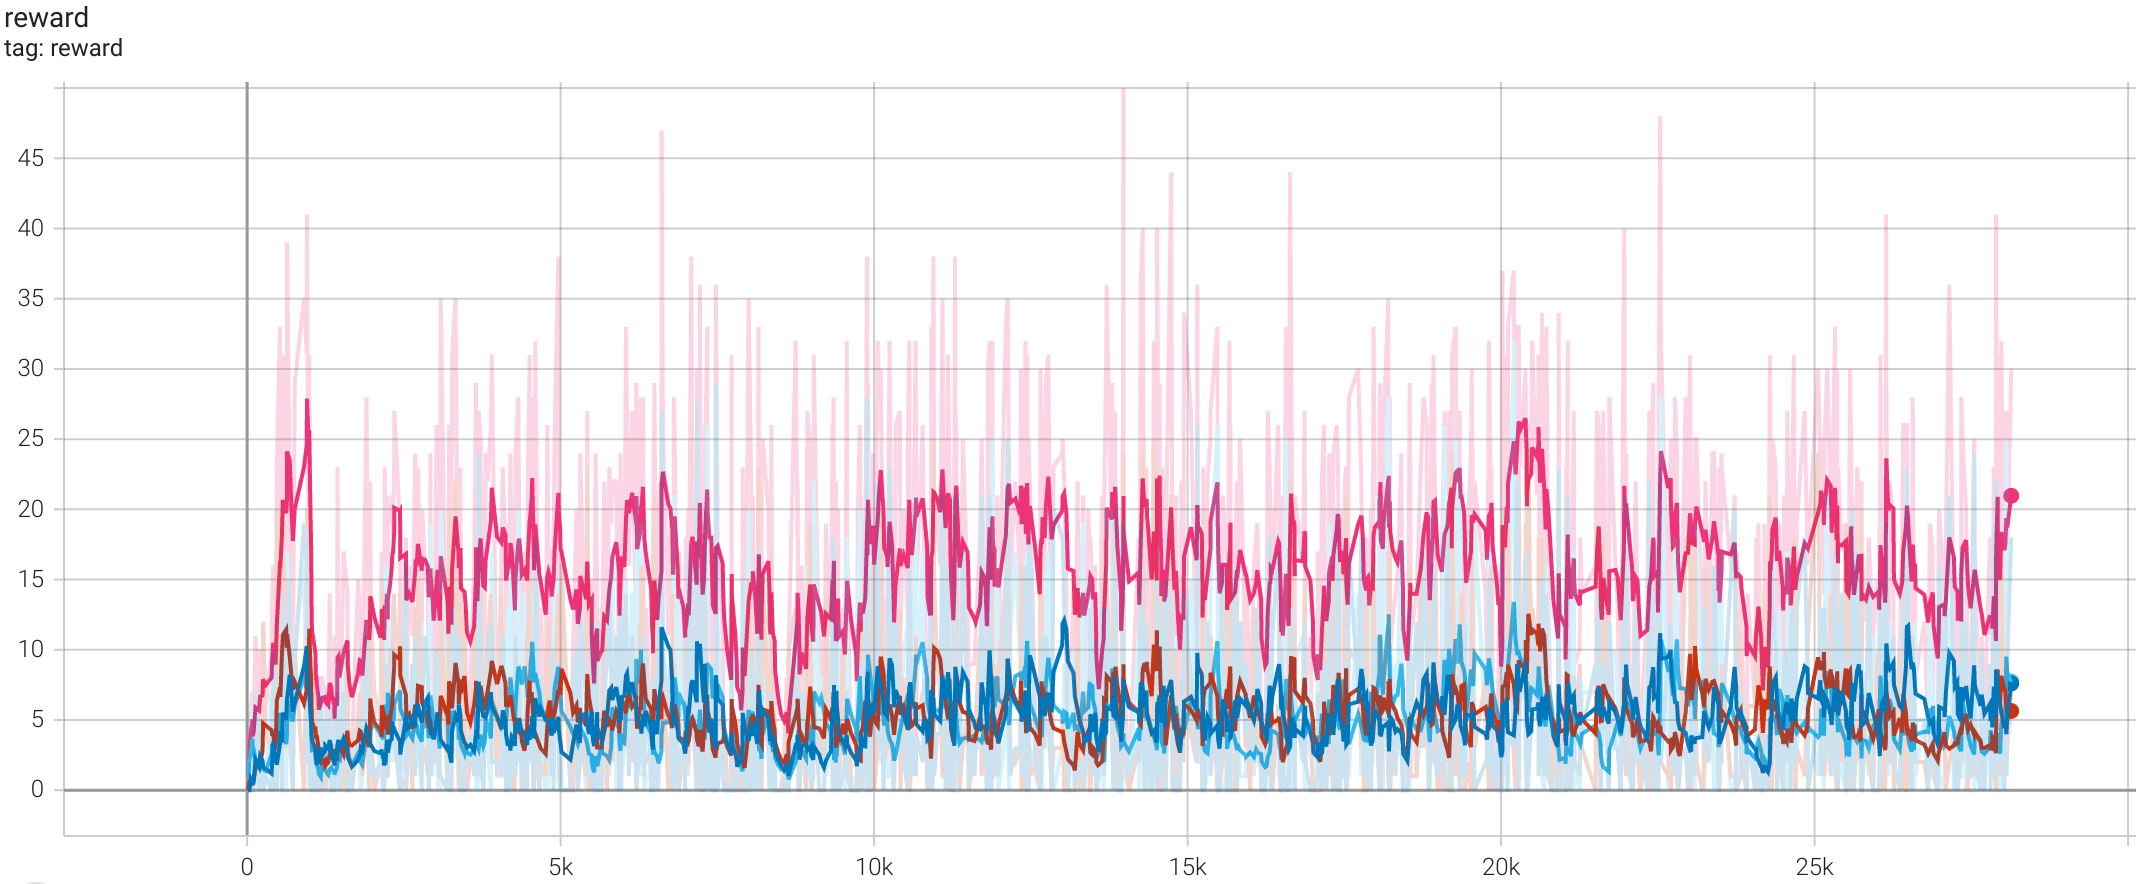
\includegraphics[width=6cm]{figs/training_reward_1.png}
        \caption{Reward during training}
        \label{rw1}
    \end{minipage}
    \begin{minipage}[t]{0.48\textwidth}
        \centering
        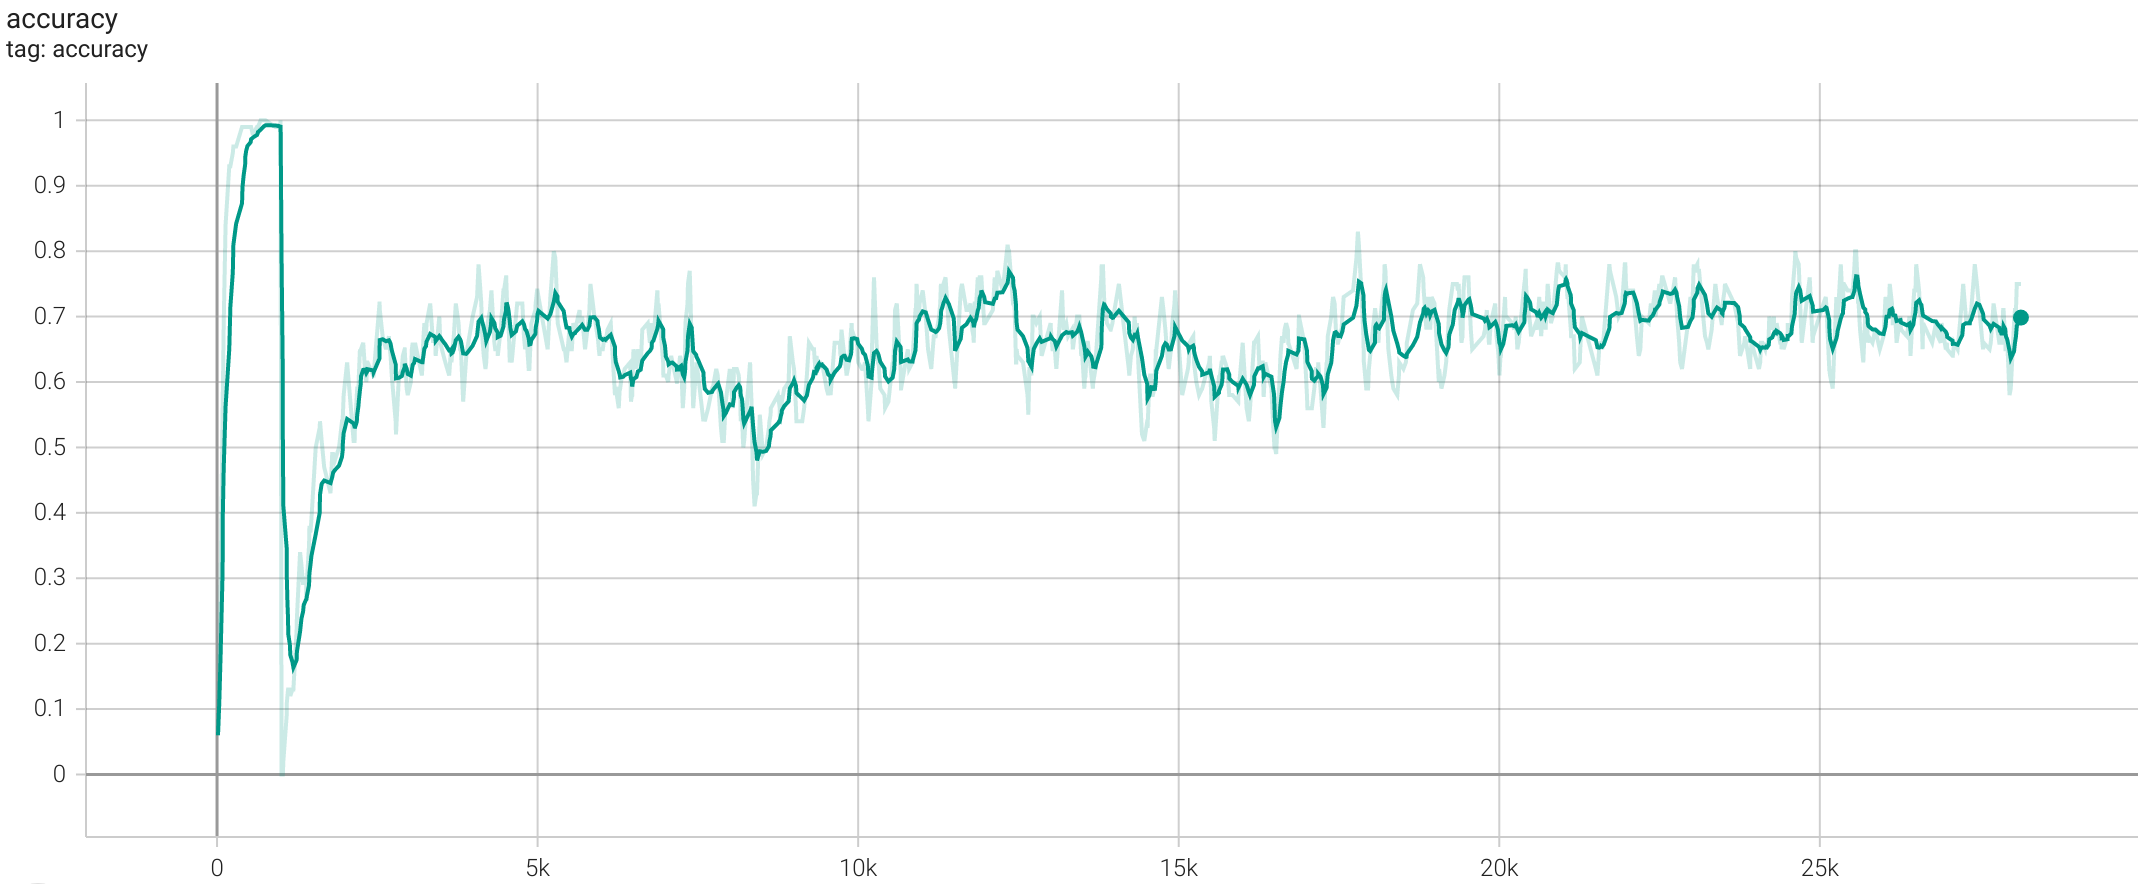
\includegraphics[width=6cm]{figs/training_win_rate_1.png}
        \caption{Win rate during training}
        \label{wr1}
    \end{minipage}
\end{figure}

In another attempt, we use VI agent to train it directly. The reward and win rate during training are shown in figure \ref{rw2} and figure \ref{wr2}.

\begin{figure}[H]
    \centering
    \begin{minipage}[t]{0.48\textwidth}
        \centering
        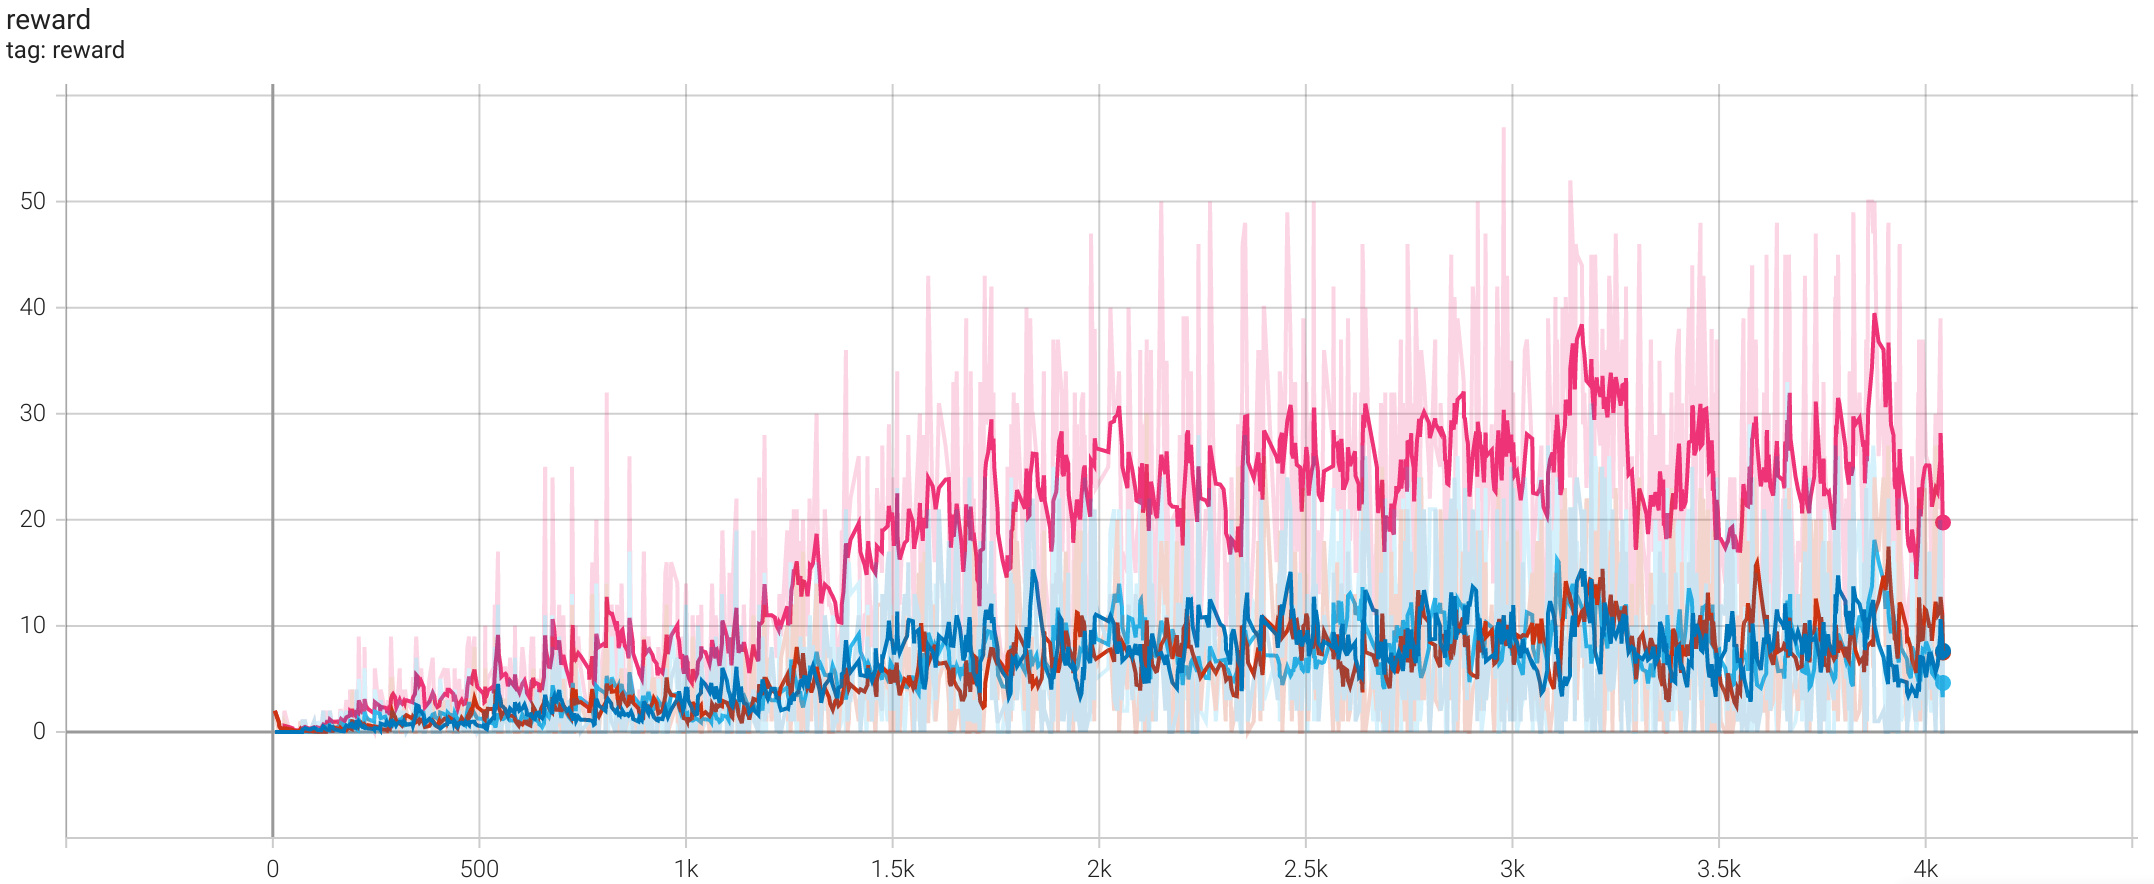
\includegraphics[width=6cm]{figs/training_reward.png}
        \caption{Reward during training}
        \label{rw2}
    \end{minipage}
    \begin{minipage}[t]{0.48\textwidth}
        \centering
        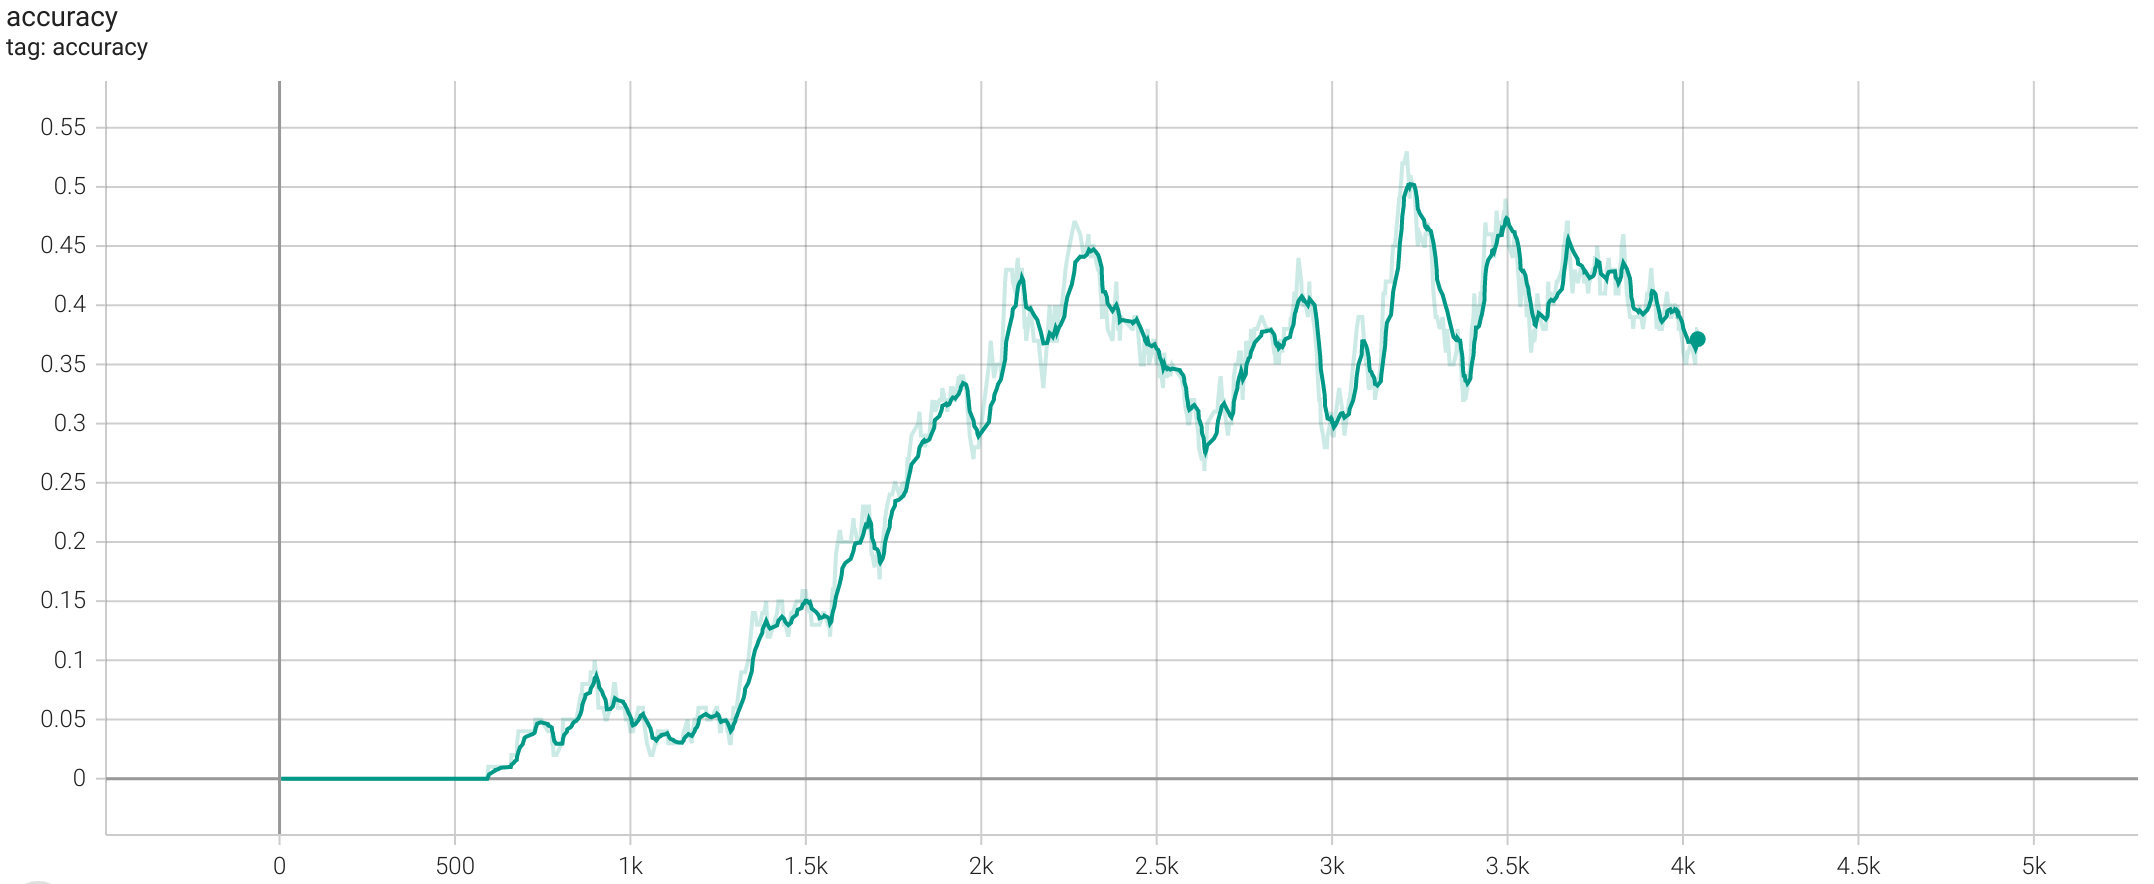
\includegraphics[width=6cm]{figs/training_win_rate.png}
        \caption{Win rate during training}
        \label{wr2}
    \end{minipage}
\end{figure}

\subsection{Result}
Its final performance is shown in figure \ref{dqn-rl}. Here we use Value Iteration agent to be the opponent during training the Dueling DQN model. And we train for 4,000 episodes.

\begin{figure}[H]
  \centering
  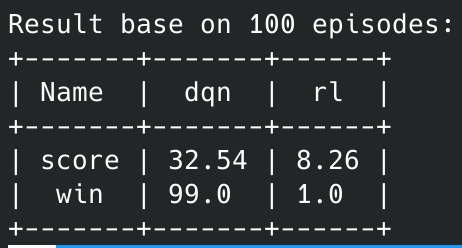
\includegraphics[width=0.5\textwidth]{figs/dqn_vs_rl.png}
  \caption{Dueling DQN agent with RL agent}
  \label{dqn-rl}
\end{figure}

\section{Analysis}

\subsection{Advantages and disadvantages}

\begin{table}[H]
  \caption{Advantages and disadvantages of 3 algorithms}
  \label{pros-cons}
  \centering
  \begin{tabular}{llll}
    \toprule
    Name & Implementation & Space needed & Performance \\
    \midrule
    Minimax with $\alpha$-$\beta$ Pruning & Simple and intuitive & Large & Bad \\
    Value Iteration \& Policy Iteration & Simple and intuitive & Small & Decent \\
    Dueling DQN     & Relatively complex & Small & \makecell{Maybe the best \\ (If well-trained)} \\
    \bottomrule
  \end{tabular}
\end{table}

As shown in table \ref{pros-cons}, the 3 algorithms we have tried in this project have their advantages and disadvantages. 

\subsection{Comparison of VI and DQN}

Although our DQN agent performed better against the RL agent, it was still the underdog against the intuitive VI agent. We think there may be several reasons for this.
\begin{enumerate}
    \item The main reason is that we were not able to find better training parameters, resulting in unsatisfactory training results. As we know, tuning parameters is an important part of training models, which can directly affect the training rate and accuracy of the model. However, due to our lack of experience and the long time required for training, we were unable to find good training parameters.
    \item At the same time, we use more special strategies in the VI agent. This is simple and straightforward, but also very effective. However, we cannot make the Dueling DQN agent acquire these strategies by directly adjusting the neural network structure, but we can only hope that it will acquire them by itself. This process is full of uncertainty, and as a result, it fails to acquire these strategies.
\end{enumerate}

\subsection{Final agent}
Due to the reasons above, we choose VI agent as our final agent. Its performance on the public channel\footnote{http://www.jidiai.cn/ranking\_list?tab=6} is shown in figure \ref{jidi_vi}.
\begin{figure}[H]
  \centering
  
\includegraphics[width=1\textwidth]{figs/vi_on_jidi.png}
  \caption{VI agent on Jidi platform}
  \label{jidi_vi}
\end{figure}

\section{Summary}

In completing this project, we both learned a lot while deepening our understanding of what we had learned in class. We tried several algorithms to solve the problem based on the analysis of the problem and from what we learned in class. The VI agent we designed on the first day already had good results, but we were not satisfied with that and continued to explore in two directions: on the one hand, we improved the performance of the VI agent by adding specific strategies, and on the other hand, we tried more complex Dueling DQN algorithms.

Although we were not able to find better training parameters for the DQN algorithm in the end, we learned a lot about deep learning and reinforcement learning in our continuous attempts, so these attempts are worthwhile.

In the end, we still chose the enhanced VI agent as the submission for the final competition because its intuitive algorithm was sufficient for most of the opponents.

% \section{Headings: first level}
% \label{headings}

% All headings should be lower case (except for first word and proper nouns),
% flush left, and bold.

% First-level headings should be in 12-point type.

% \subsection{Headings: second level}

% Second-level headings should be in 10-point type.

% \subsubsection{Headings: third level}

% Third-level headings should be in 10-point type.

% \paragraph{Paragraphs}

% There is also a \verb+\paragraph+ command available, which sets the heading in
% bold, flush left, and inline with the text, with the heading followed by 1\,em
% of space.

% \section{Citations, figures, tables, references}
% \label{others}

% These instructions apply to everyone.

% \subsection{Citations within the text}

% The \verb+natbib+ package will be loaded for you by default.  Citations may be
% author/year or numeric, as long as you maintain internal consistency.  As to the
% format of the references themselves, any style is acceptable as long as it is
% used consistently.

% The documentation for \verb+natbib+ may be found at
% \begin{center}
%   \url{http://mirrors.ctan.org/macros/latex/contrib/natbib/natnotes.pdf}
% \end{center}
% Of note is the command \verb+\citet+, which produces citations appropriate for
% use in inline text.  For example,
% \begin{verbatim}
%   \citet{hasselmo} investigated\dots
% \end{verbatim}
% produces
% \begin{quote}
%   Hasselmo, et al.\ (1995) investigated\dots
% \end{quote}

% If you wish to load the \verb+natbib+ package with options, you may add the
% following before loading the \verb+neurips_2021+ package:
% \begin{verbatim}
%   \PassOptionsToPackage{options}{natbib}
% \end{verbatim}

% If \verb+natbib+ clashes with another package you load, you can add the optional
% argument \verb+nonatbib+ when loading the style file:
% \begin{verbatim}
%   \usepackage[nonatbib]{neurips_2021}
% \end{verbatim}

% As submission is double blind, refer to your own published work in the third
% person. That is, use ``In the previous work of Jones et al.\ [4],'' not ``In our
% previous work [4].'' If you cite your other papers that are not widely available
% (e.g., a journal paper under review), use anonymous author names in the
% citation, e.g., an author of the form ``A.\ Anonymous.''

% \subsection{Footnotes}

% Footnotes should be used sparingly.  If you do require a footnote, indicate
% footnotes with a number\footnote{Sample of the first footnote.} in the
% text. Place the footnotes at the bottom of the page on which they appear.
% Precede the footnote with a horizontal rule of 2~inches (12~picas).

% Note that footnotes are properly typeset \emph{after} punctuation
% marks.\footnote{As in this example.}

% \subsection{Figures}

% \begin{figure}
%   \centering
%   \fbox{\rule[-.5cm]{0cm}{4cm} \rule[-.5cm]{4cm}{0cm}}
%   \caption{Sample figure caption.}
% \end{figure}

% All artwork must be neat, clean, and legible. Lines should be dark enough for
% purposes of reproduction. The figure number and caption always appear after the
% figure. Place one line space before the figure caption and one line space after
% the figure. The figure caption should be lower case (except for first word and
% proper nouns); figures are numbered consecutively.

% You may use color figures.  However, it is best for the figure captions and the
% paper body to be legible if the paper is printed in either black/white or in
% color.

% \subsection{Tables}

% All tables must be centered, neat, clean and legible.  The table number and
% title always appear before the table.  See Table~\ref{sample-table}.

% Place one line space before the table title, one line space after the
% table title, and one line space after the table. The table title must
% be lower case (except for first word and proper nouns); tables are
% numbered consecutively.

% Note that publication-quality tables \emph{do not contain vertical rules.} We
% strongly suggest the use of the \verb+booktabs+ package, which allows for
% typesetting high-quality, professional tables:
% \begin{center}
%   \url{https://www.ctan.org/pkg/booktabs}
% \end{center}
% This package was used to typeset Table~\ref{sample-table}.

% \begin{table}
%   \caption{Sample table title}
%   \label{sample-table}
%   \centering
%   \begin{tabular}{lll}
%     \toprule
%     \multicolumn{2}{c}{Part}                   \\
%     \cmidrule(r){1-2}
%     Name     & Description     & Size ($\mu$m) \\
%     \midrule
%     Dendrite & Input terminal  & $\sim$100     \\
%     Axon     & Output terminal & $\sim$10      \\
%     Soma     & Cell body       & up to $10^6$  \\
%     \bottomrule
%   \end{tabular}
% \end{table}

% \section{Final instructions}

% Do not change any aspects of the formatting parameters in the style files.  In
% particular, do not modify the width or length of the rectangle the text should
% fit into, and do not change font sizes (except perhaps in the
% \textbf{References} section; see below). Please note that pages should be
% numbered.

% \section{Preparing PDF files}

% Please prepare submission files with paper size ``US Letter,'' and not, for
% example, ``A4.''

% Fonts were the main cause of problems in the past years. Your PDF file must only
% contain Type 1 or Embedded TrueType fonts. Here are a few instructions to
% achieve this.

% \begin{itemize}

% \item You should directly generate PDF files using \verb+pdflatex+.

% \item You can check which fonts a PDF files uses.  In Acrobat Reader, select the
%   menu Files$>$Document Properties$>$Fonts and select Show All Fonts. You can
%   also use the program \verb+pdffonts+ which comes with \verb+xpdf+ and is
%   available out-of-the-box on most Linux machines.

% \item The IEEE has recommendations for generating PDF files whose fonts are also
%   acceptable for NeurIPS. Please see
%   \url{http://www.emfield.org/icuwb2010/downloads/IEEE-PDF-SpecV32.pdf}

% \item \verb+xfig+ "patterned" shapes are implemented with bitmap fonts.  Use
%   "solid" shapes instead.

% \item The \verb+\bbold+ package almost always uses bitmap fonts.  You should use
%   the equivalent AMS Fonts:
% \begin{verbatim}
%   \usepackage{amsfonts}
% \end{verbatim}
% followed by, e.g., \verb+\mathbb{R}+, \verb+\mathbb{N}+, or \verb+\mathbb{C}+
% for $\mathbb{R}$, $\mathbb{N}$ or $\mathbb{C}$.  You can also use the following
% workaround for reals, natural and complex:
% \begin{verbatim}
%   \newcommand{\RR}{I\!\!R} %real numbers
%   \newcommand{\Nat}{I\!\!N} %natural numbers
%   \newcommand{\CC}{I\!\!\!\!C} %complex numbers
% \end{verbatim}
% Note that \verb+amsfonts+ is automatically loaded by the \verb+amssymb+ package.

% \end{itemize}

% If your file contains type 3 fonts or non embedded TrueType fonts, we will ask
% you to fix it.

% \subsection{Margins in \LaTeX{}}

% Most of the margin problems come from figures positioned by hand using
% \verb+\special+ or other commands. We suggest using the command
% \verb+\includegraphics+ from the \verb+graphicx+ package. Always specify the
% figure width as a multiple of the line width as in the example below:
% \begin{verbatim}
%   \usepackage[pdftex]{graphicx} ...
%   \includegraphics[width=0.8\linewidth]{myfile.pdf}
% \end{verbatim}
% See Section 4.4 in the graphics bundle documentation
% (\url{http://mirrors.ctan.org/macros/latex/required/graphics/grfguide.pdf})

% A number of width problems arise when \LaTeX{} cannot properly hyphenate a
% line. Please give LaTeX hyphenation hints using the \verb+\-+ command when
% necessary.

\begin{ack}
We would like to thank Prof. Shuai Li and teaching assistants for their guidance and help throughout the semester. We have learned a lot in CS410 Artificial Intelligence course\footnote{https://shuaili8.github.io/Teaching/CS410/index.html} and have developed a strong interest in AI.
\end{ack}

\section*{References}

{
\small

[1] Russell, S., \& Norvig, P. (2002). Artificial intelligence: a modern approach.

[2] Sutton, R. S., \& Barto, A. G. (2018). Reinforcement learning: An introduction. MIT press.

[3] Zhou, Z. H. (2021). Machine learning. Springer.

[4] Mnih, V., Kavukcuoglu, K., Silver, D., Graves, A., Antonoglou, I., Wierstra, D., \& Riedmiller, M. (2013). Playing atari with deep reinforcement learning. arXiv preprint arXiv:1312.5602.

[5] Mnih, V., Kavukcuoglu, K., Silver, D., Rusu, A. A., Veness, J., Bellemare, M. G., ... \& Hassabis, D. (2015). Human-level control through deep reinforcement learning. nature, 518(7540), 529-533.

[6] Wang, Z., Schaul, T., Hessel, M., Hasselt, H., Lanctot, M., \& Freitas, N. (2016, June). Dueling network architectures for deep reinforcement learning. In International conference on machine learning (pp. 1995-2003). PMLR.
}

%%%%%%%%%%%%%%%%%%%%%%%%%%%%%%%%%%%%%%%%%%%%%%%%%%%%%%%%%%%%
% \section*{Checklist}

% %%% BEGIN INSTRUCTIONS %%%
% The checklist follows the references.  Please
% read the checklist guidelines carefully for information on how to answer these
% questions.  For each question, change the default \answerTODO{} to \answerYes{},
% \answerNo{}, or \answerNA{}.  You are strongly encouraged to include a {\bf
% justification to your answer}, either by referencing the appropriate section of
% your paper or providing a brief inline description.  For example:
% \begin{itemize}
%   \item Did you include the license to the code and datasets? \answerYes{See Section~\ref{gen_inst}.}
%   \item Did you include the license to the code and datasets? \answerNo{The code and the data are proprietary.}
%   \item Did you include the license to the code and datasets? \answerNA{}
% \end{itemize}
% Please do not modify the questions and only use the provided macros for your
% answers.  Note that the Checklist section does not count towards the page
% limit.  In your paper, please delete this instructions block and only keep the
% Checklist section heading above along with the questions/answers below.
% %%% END INSTRUCTIONS %%%

% \begin{enumerate}

% \item For all authors...
% \begin{enumerate}
%   \item Do the main claims made in the abstract and introduction accurately reflect the paper's contributions and scope?
%     \answerTODO{}
%   \item Did you describe the limitations of your work?
%     \answerTODO{}
%   \item Did you discuss any potential negative societal impacts of your work?
%     \answerTODO{}
%   \item Have you read the ethics review guidelines and ensured that your paper conforms to them?
%     \answerTODO{}
% \end{enumerate}

% \item If you are including theoretical results...
% \begin{enumerate}
%   \item Did you state the full set of assumptions of all theoretical results?
%     \answerTODO{}
% 	\item Did you include complete proofs of all theoretical results?
%     \answerTODO{}
% \end{enumerate}

% \item If you ran experiments...
% \begin{enumerate}
%   \item Did you include the code, data, and instructions needed to reproduce the main experimental results (either in the supplemental material or as a URL)?
%     \answerTODO{}
%   \item Did you specify all the training details (e.g., data splits, hyperparameters, how they were chosen)?
%     \answerTODO{}
% 	\item Did you report error bars (e.g., with respect to the random seed after running experiments multiple times)?
%     \answerTODO{}
% 	\item Did you include the total amount of compute and the type of resources used (e.g., type of GPUs, internal cluster, or cloud provider)?
%     \answerTODO{}
% \end{enumerate}

% \item If you are using existing assets (e.g., code, data, models) or curating/releasing new assets...
% \begin{enumerate}
%   \item If your work uses existing assets, did you cite the creators?
%     \answerTODO{}
%   \item Did you mention the license of the assets?
%     \answerTODO{}
%   \item Did you include any new assets either in the supplemental material or as a URL?
%     \answerTODO{}
%   \item Did you discuss whether and how consent was obtained from people whose data you're using/curating?
%     \answerTODO{}
%   \item Did you discuss whether the data you are using/curating contains personally identifiable information or offensive content?
%     \answerTODO{}
% \end{enumerate}

% \item If you used crowdsourcing or conducted research with human subjects...
% \begin{enumerate}
%   \item Did you include the full text of instructions given to participants and screenshots, if applicable?
%     \answerTODO{}
%   \item Did you describe any potential participant risks, with links to Institutional Review Board (IRB) approvals, if applicable?
%     \answerTODO{}
%   \item Did you include the estimated hourly wage paid to participants and the total amount spent on participant compensation?
%     \answerTODO{}
% \end{enumerate}

% \end{enumerate}

%%%%%%%%%%%%%%%%%%%%%%%%%%%%%%%%%%%%%%%%%%%%%%%%%%%%%%%%%%%%
\clearpage

\appendix

\section{Role and contribution of each member in the group}

\begin{multicols}{2}
Keyao You: \textbf{60\%}.
\begin{itemize}
    \item Most of the code;
    \item Model training and testing;
    \item Report writing.
\end{itemize}

\quad

Yazhou Tang: \textbf{40\%}.
\begin{itemize}
    \item Least of the code;
    \item Model training and testing;
    \item Presentation;
    \item Report writing.
\end{itemize}
\end{multicols}

\section{Code}

You can see the full code on https://github.com/youkeyao/SJTU-CS410-Snakes-3V3-Group06.


% Additionally, please identify the role of each member in the group and the
% corresponding contribution percentage.

\end{document}